\documentclass{article}
\usepackage{gensymb, amsmath, float, graphicx, epstopdf}
\restylefloat{table}
\usepackage[margin=0.75in]{geometry}
\begin{document}

\title{Lab Write-up 4: Shielded-Loop Resonators}
\author{Michael Shen}
\maketitle


\section{Finding the Resonant Frequency}

\subsection{Measured Data}

\begin{table}[H]
\centering
\begin{tabular}{|c|c|c|}
\hline
Loop & $f_0$ (MHz) & $\vert\Gamma^{\prime}_{in}\vert$ \\ \hline
5 cm & 89.209 & 0.237 \\ \hline
9 cm & 49.774 & 0.260 \\ \hline
\end{tabular}
\end{table}

\subsection{Questions}

\begin{enumerate}
	\item Since $C \approx C^{\prime}l$, the longer, 9 cm, loop should have a greater capacitance.
	\item Since $L = \mu r [ln \frac{32r}{d}-1.75]$ for shielded-loop resonators and $\mu$ and $d$ are constant between the loops, the loop with the larger radius, the 9 cm loop, should have a greater inductance.
	\item Since $f_0 = \dfrac{\omega_0}{2\pi}$ and $\omega_0 = \dfrac{1}{\sqrt{LC}}$, the loop with the smaller $LC$ product will have a higher resonant frequency. Since the 5cm loop should have both a smaller $C$ and $L$, it should have a higher resonant frequency. This is confirmed by our experimental results as the 5 cm loop has a resonant frequency of 89.209 MHz compared to a resonant frequency of 49.774 MHz for the 9 cm loop.
\end{enumerate}


\section{De-embedding the Feedline}

\subsection{Measured Data}
\begin{table}[H]
\centering
\begin{tabular}{|c|c|c|c|}
\hline
Loop & $\vert\Gamma^{\prime}_{in}\vert$ & $\vert\Gamma^{\prime}_{in}\vert$ at $f_0$ - 2MHz & $\vert\Gamma^{\prime}_{in}\vert$ at $f_0$ + 2MHz \\ \hline
5 cm & 0.9735\angle 109.9\degree & 0.9745\angle 123.5\degree & 0.9744\angle 96.61\degree \\ \hline
9 cm & 0.9712\angle 118.1\degree & 0.9745\angle 143.6\degree & 0.9772\angle 93.61\degree \\ \hline
\end{tabular}
\end{table}

\subsection{Analysis}
\begin{enumerate}
	\item $\beta l$ 5cm line: $\dfrac{((123.5-109.9)+(109.9-96.61))}{2}= 13.45\degree = 0.2347$ \\
		  $\beta l$ 9cm line: $\dfrac{((143.6-118.1)+(118.1-93.61))}{2}= 25.00\degree = 0.4362$ \\
	\item $\beta l$ 5cm line at $f_0 - 2$MHz: $\beta l\frac{f_0 - 2}{f_0} = 0.225$\\
		  $\beta l$ 5cm line at $f_0 + 2$MHz: $\beta l\frac{f_0 + 2}{f_0} = 0.244$\\
		  $\beta l$ 9cm line at $f_0 - 2$MHz: $\beta l\frac{f_0 - 2}{f_0} = 0.426$\\
		  $\beta l$ 9cm line at $f_0 + 2$MHz: $\beta l\frac{f_0 + 2}{f_0} = 0.446$\\
	\item 
	\item 
	\item 
\end{enumerate}

\subsection{Questions}
\begin{enumerate}
	\item 
	\item 
\end{enumerate}


\section{Finding R, L, and C}

\subsection{Measured Data}
\begin{table}[H]
\centering
\begin{tabular}{|l|l|l|l|}
\hline
Loop & R & L & C \\ \hline
5 cm &   &   &  \\ \hline
9 cm &   &   &  \\ \hline
\end{tabular}
\end{table}

\subsection{Analysis}

\begin{enumerate}
	\item
	\item
\end{enumerate}

\subsection{Questions}

\begin{enumerate}
	\item 
	\item 
	\item 
\end{enumerate}

%\section{Figures and Images}
%\begin{figure}[H]
%    \centering
%    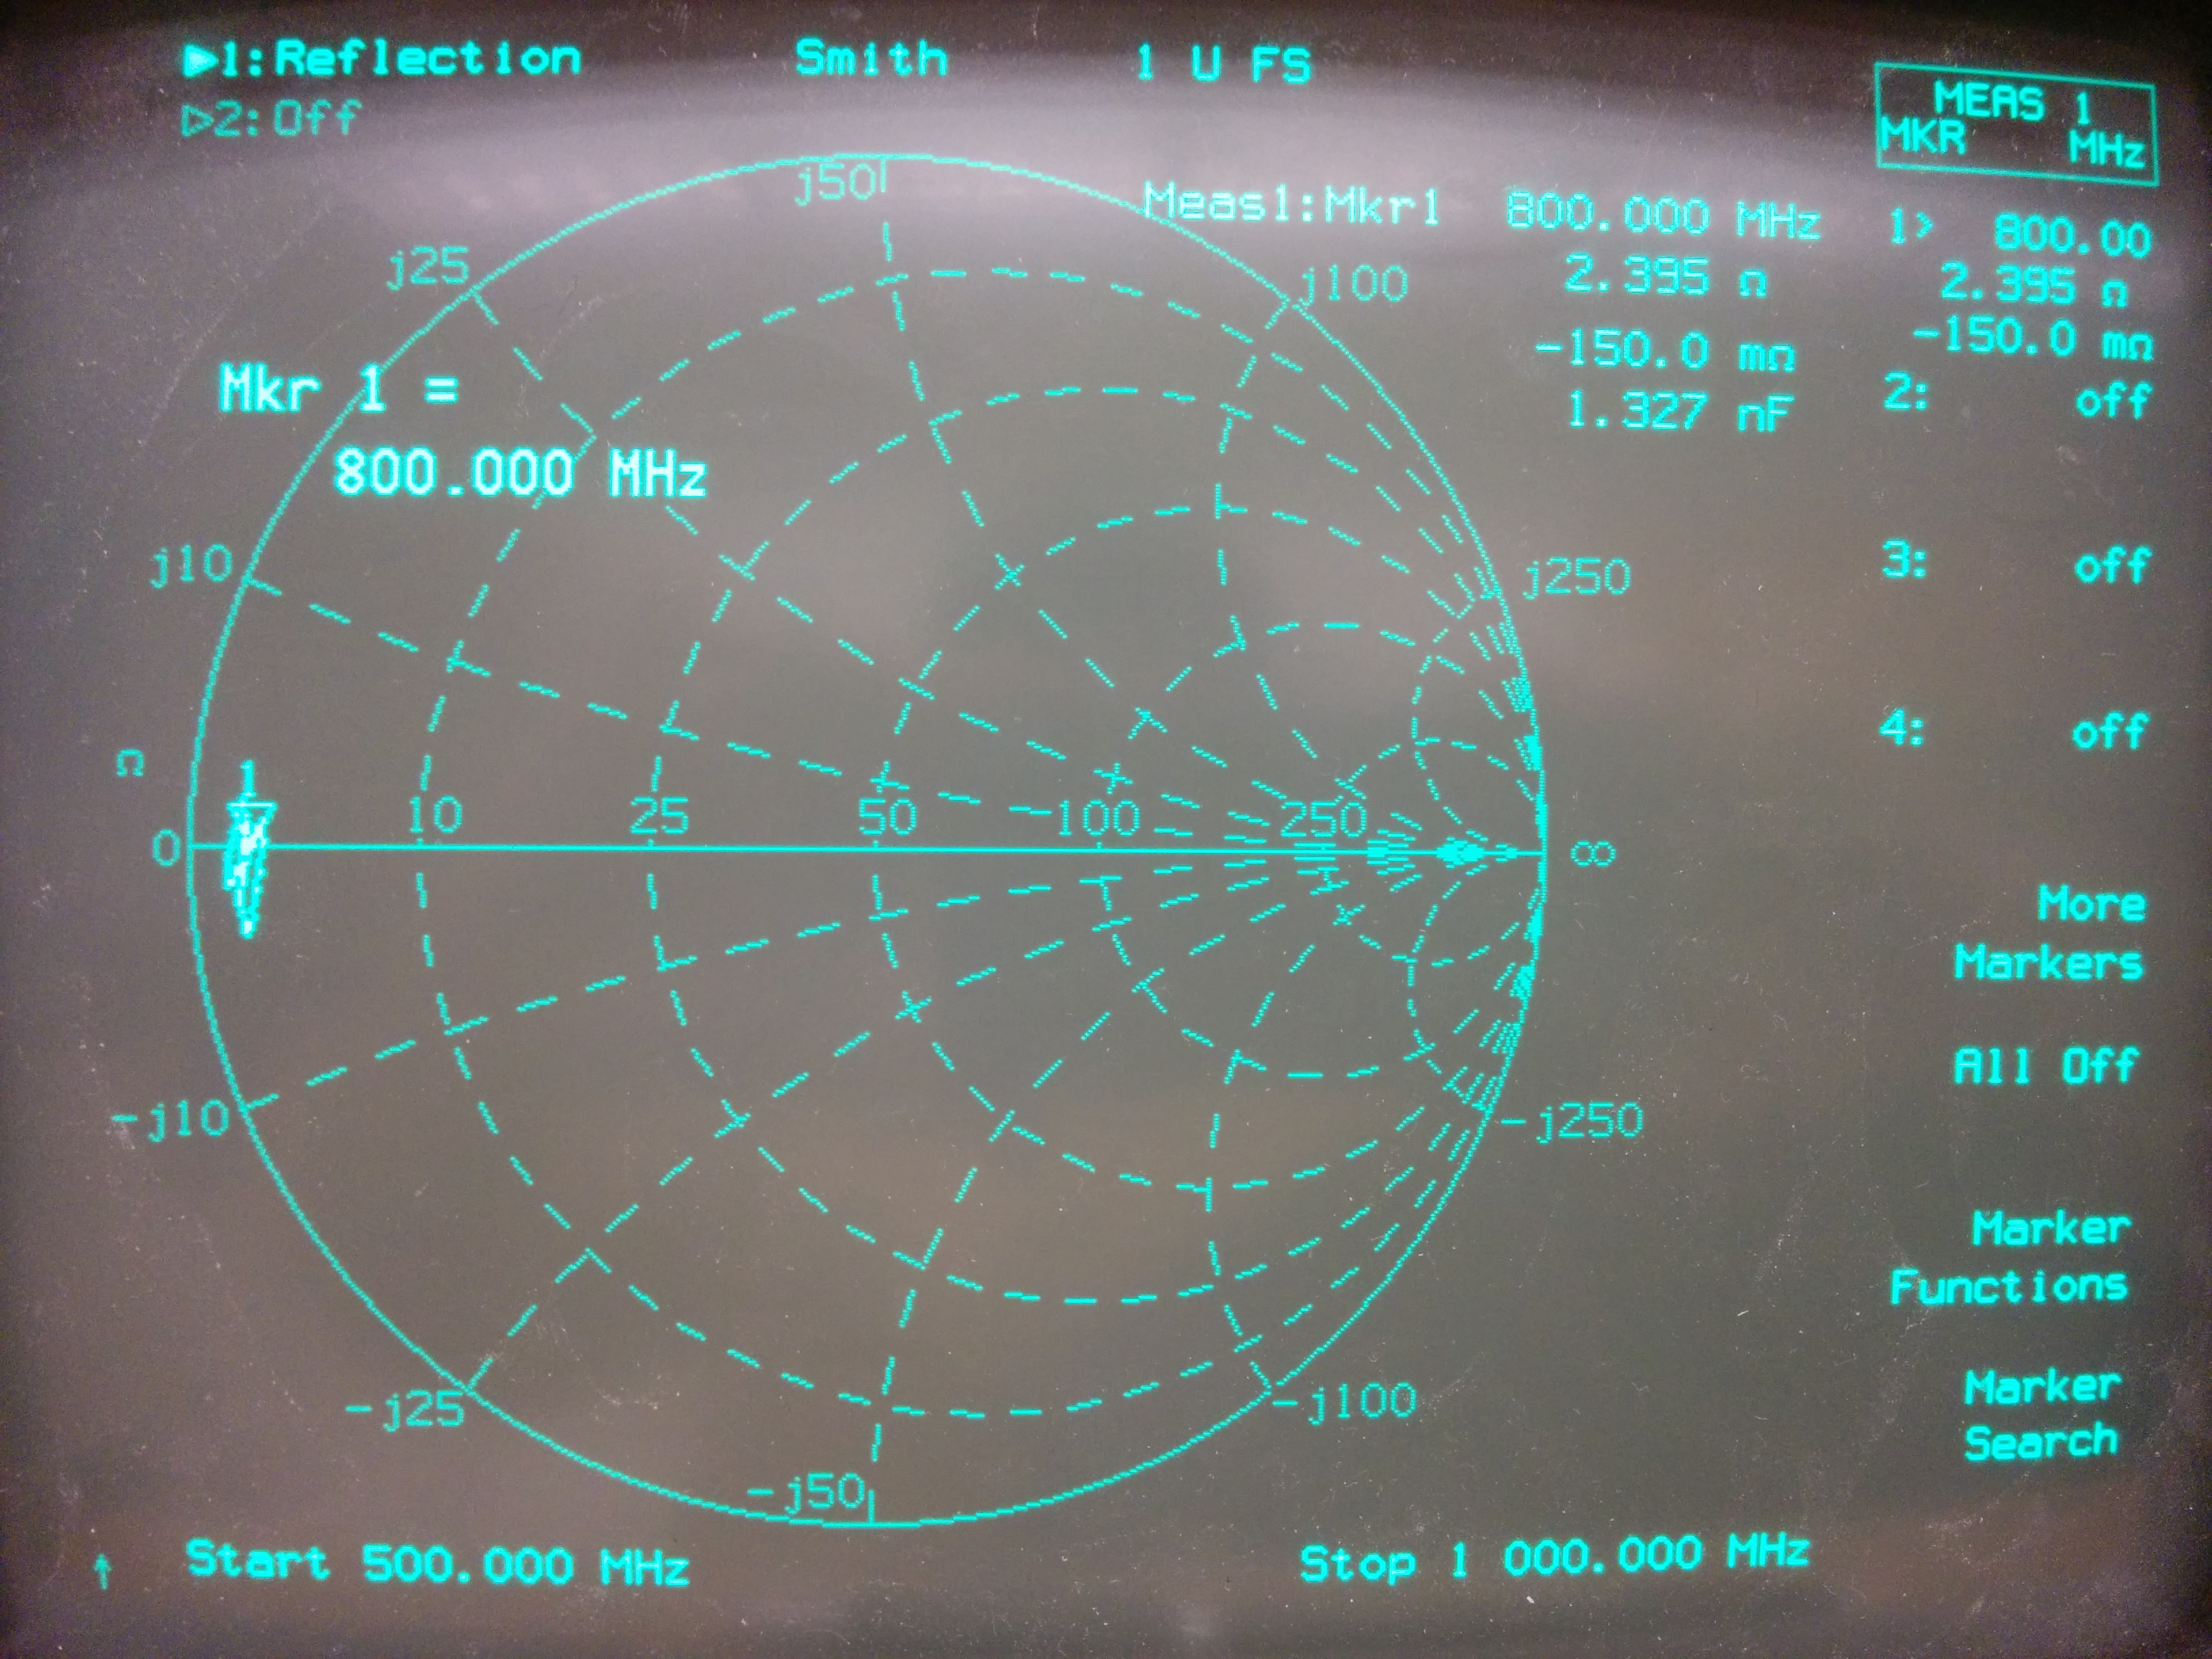
\includegraphics[width=0.8\textwidth]{./Images/251.jpg}
%    \caption{Point-like response for a lossless line}
%\end{figure}

\end{document}